\documentclass[table,german,10pt]{beamer}
\usepackage[utf8]{luainputenc}
\usepackage{tcs-lecture}
\usepackage{yfonts}
\usepackage{appendixnumberbeamer}

\usetikzlibrary{arrows, shapes}
\tikzstyle{edge} = [fill,opacity=.5,fill opacity=.5,line cap=round, line
join=round, line width=50pt]
% \input{../config/lecture-config.tex}
\DeclareMathOperator{\perm}{perm}
\author{Sebastian Berndt}
\setbeamertemplate{sidebar right}{}
\setbeamertemplate{title page}
{
  \vbox{}
  \ifcd\vskip-5mm\leavevmode\hbox{\hskip-3mm\includegraphics[scale=0.45]{uzl-logo-ITCS.pdf}}%
  \par
  \leftskip3mm\else
  \vskip1em\fi
  {\huge \insertshortlecture\par}
  {\usebeamercolor[fg]{title}\usebeamerfont{title}\inserttitle\par}%
  \ifx\insertsubtitle\@empty%
  \else%
  \vskip0.25em%
  {\usebeamerfont{subtitle}\usebeamercolor[fg]{subtitle}\insertsubtitle\par}%
  \fi%     
  \vskip4pt\par
  \usebeamercolor[fg]{author}\insertauthor
  \ifcd\vskip1em
  {\centering \scalebox{2}{\hbox{\insertlogo}}}
  \vskip0pt plus1filll\else
  \insertinstitute\vskip1em\fi
}

\logo{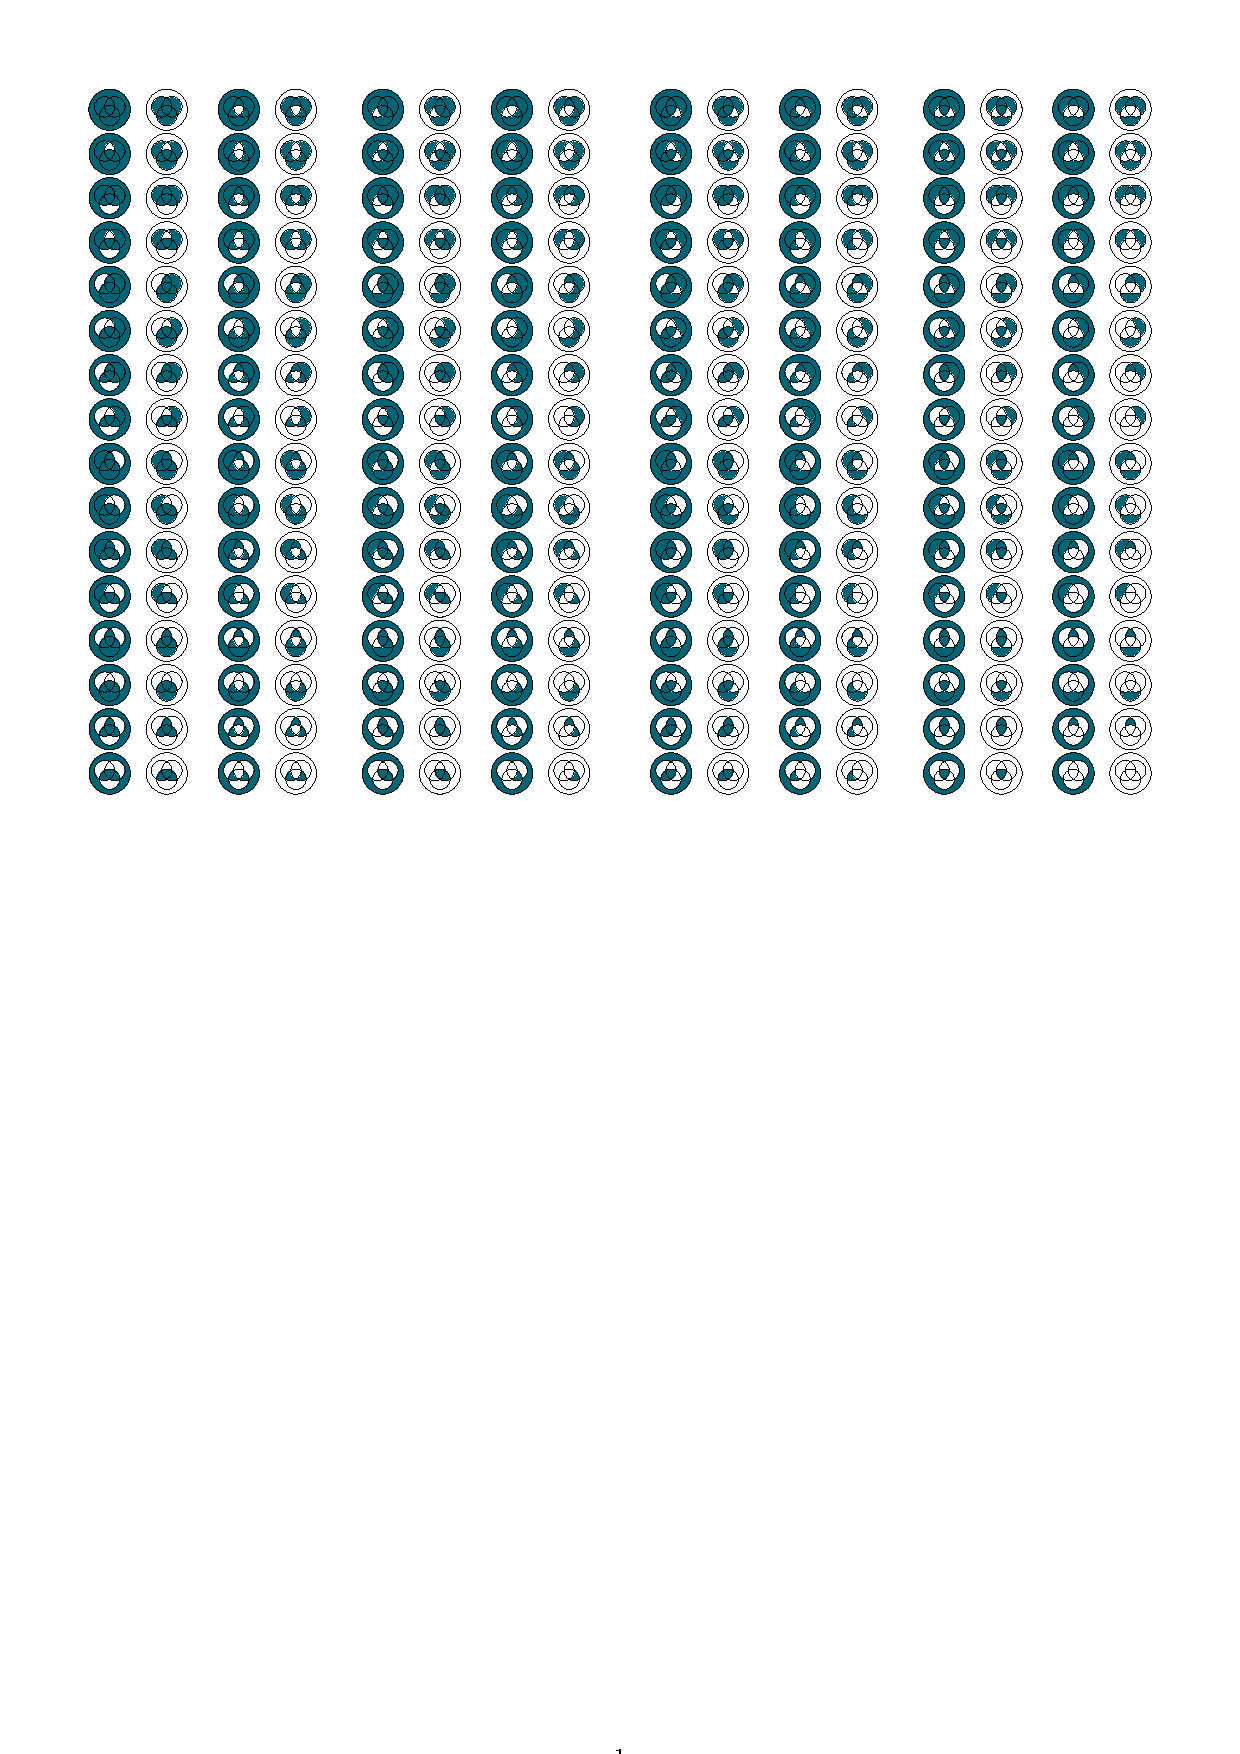
\includegraphics[scale=0.17]{logo}
}

\newcommand{\regionA}[1]
{   \fill[#1] (30:2) arc (60:0:{2*sqrt(3)}) arc (-60:120:{2*sqrt(3)}) arc (60:0:{2*sqrt(3)});
}

\newcommand{\regionB}[1]
{   \fill[#1] (150:2) arc (180:120:{2*sqrt(3)}) arc (60:240:{2*sqrt(3)}) arc (180:120:{2*sqrt(3)});
}

\newcommand{\regionC}[1]
{   \fill[#1] (270:2) arc (240:300:{2*sqrt(3)}) arc (360:180:{2*sqrt(3)}) arc (240:300:{2*sqrt(3)});
}

\newcommand{\regionAB}[1]
{   \fill[#1] (30:2) arc (0:60:{2*sqrt(3)}) arc (120:180:{2*sqrt(3)}) arc (120:60:{2*sqrt(3)});
}

\newcommand{\regionAC}[1]
{   \fill[#1] (30:2) arc (60:0:{2*sqrt(3)}) arc (300:240:{2*sqrt(3)}) arc (-60:0:{2*sqrt(3)});
}

\newcommand{\regionBC}[1]
{   \fill[#1] (150:2) arc (120:180:{2*sqrt(3)}) arc (240:300:{2*sqrt(3)}) arc (240:180:{2*sqrt(3)});
}

\newcommand{\regionABC}[1]
{   \fill[#1] (30:2) arc (60:120:{2*sqrt(3)}) arc (180:240:{2*sqrt(3)}) arc (-60:0:{2*sqrt(3)});
}

\newcommand{\regionDarkside}[1]
{   \fill[#1,even odd rule] (90:4) arc (120:-60:{2*sqrt(3)}) arc (360:180:{2*sqrt(3)}) arc (240:60:{2*sqrt(3)}) (0,0) circle (7);
}


\def\insertlecture{Oberseminar}
\lecture{Inclusion-Exclusion}{in-ex}
\begin{document}


\maketitle
\begin{frame}{Ausgangssituation}
  \begin{columns}
    \begin{column}{5.5cm}
      \only<1>{
        \begin{tikzpicture}[scale=0.35]
          \node {M};
          \draw (0,0) circle (7);
          \clip (0,0) circle (7);
          \useasboundingbox (0,0) circle (7);

        \end{tikzpicture}      
      }
      \only<2>{
        \begin{tikzpicture}[scale=0.35]
          \regionA{white}
          \regionB{white}
          \regionC{white}
          \regionAB{white}
          \regionAC{white}
          \regionBC{white}
          \regionABC{white}
          \regionDarkside{white}
          \draw (30:2) node[xshift=1cm] {$P_{1}$} circle ({2*sqrt(3)});
          \draw (150:2) node[xshift=-1cm] {$P_{2}$} circle ({2*sqrt(3)});
          \draw (270:2) node[yshift=-1cm] {$P_{3}$} circle ({2*sqrt(3)});
          \draw (0,0) circle (7);
          \clip (0,0) circle (7);
          \useasboundingbox (0,0) circle (7);
        \end{tikzpicture}      
      }
      \only<3>{
        \begin{tikzpicture}[scale=0.35]
          \regionA{structure.fg}
          \regionB{white}
          \regionC{white}
          \regionAB{white}
          \regionAC{white}
          \regionBC{white}
          \regionABC{white}
          \regionDarkside{structure.fg}
          \draw (30:2) node[xshift=1cm] {$P_{1}$} circle ({2*sqrt(3)});
          \draw (150:2) node[xshift=-1cm] {$P_{2}$} circle ({2*sqrt(3)});
          \draw (270:2) node[yshift=-1cm] {$P_{3}$} circle ({2*sqrt(3)});
          \draw (0,0) circle (7);
          \clip (0,0) circle (7);
          \useasboundingbox (0,0) circle (7);
          \node[yshift=2cm] {$X(\{2,3\})$};
        \end{tikzpicture}      
      }
      \only<4,5>{
        \begin{tikzpicture}[scale=0.35]
          \regionA{white}
          \regionB{white}
          \regionC{white}
          \regionAB{white}
          \regionAC{white}
          \regionBC{white}
          \regionABC{structure.fg}
          \regionDarkside{white}
          \draw (30:2) node[xshift=1cm] {$P_{1}$} circle ({2*sqrt(3)});
          \draw (150:2) node[xshift=-1cm] {$P_{2}$} circle ({2*sqrt(3)});
          \draw (270:2) node[yshift=-1cm] {$P_{3}$} circle ({2*sqrt(3)});
          \draw (0,0) circle (7);
          \clip (0,0) circle (7);
          \useasboundingbox (0,0) circle (7);
          \node[yshift=2cm] {$M_{T}$};
        \end{tikzpicture}      
      }
    \end{column}
    \begin{column}{7cm}
      \begin{itemize}[<+->]
      \item Endliche Menge $M$
      \item Prädikate $P_{1},\ldots,P_{n}$ mit $P_{i}:M\to \{T,F\}$
      \item $X(I)=\{m\in M\ |\ P_{i}(m)=F\ \forall i\in I\}$
      \item $M_{T}=\{m\in M\ |\ P_{i}(m)=T\ \forall i\in [n]\}$
      \end{itemize}
    \end{column}
  \end{columns}
  \only<5>{
    \begin{block}{Frage}
      Wie groß ist $M_{T}$?
    \end{block}
  }
\end{frame}
% TafelBeispiel M ={1,2,3,4,5} 
\begin{frame}{Allgemeines Prinzip}
  \begin{theorem}
    \begin{align*}
      |M_{T}|=\sum_{I\subseteq [n]}(-1)^{|I|}|X(I)|
    \end{align*}
  \end{theorem}
  \pause
  \begin{block}{Anwendung}
    \begin{enumerate}[<+->]
    \item Bestimme $M$
    \item Bestimme $|X(I)|$ für festes $I$
    \item Bestimme $|M_{T}|$
    \item Laufzeit: $\mathcal{O}^{*}(2^{n})$
    \end{enumerate}
  \end{block}
\end{frame}

\begin{frame}{Ein Beispiel: Hamiltonpfad}
  \begin{columns}
    \begin{column}{5cm}
      \begin{center}
        \only<1>{
          \begin{tikzpicture}
            \tikzstyle{every node}=[thick,circle,minimum
            size=0.6cm,draw=structure.fg, fill=structure.fg!20]
            
            \node (a) {$s$};
            \node[below left = of a] (b) {$a$};
            \node[below right = of a] (c) {$b$};
            \node[below = of b] (d){$t$};
            \node[below = of c] (e){$c$};
            
            \draw[->] (a) to (e);
            \draw[->] (a) to (c);
            \draw[->] (a) to (b);
            \draw[->] (b) to (c);
            \draw[<-] (b) to (e);
            \draw[->] (c) to (d);
            \draw[->] (c) to (e);
            
          \end{tikzpicture}
        }
        \only<2-3>{
          \begin{tikzpicture}
            \tikzstyle{every node}=[thick,circle,minimum
            size=0.6cm,draw=structure.fg, fill=structure.fg!20]
            
            \node (a) {$s$};
            \node[below left = of a] (b) {$a$};
            \node[below right = of a] (c) {$b$};
            \node[below = of b] (d){$t$};
            \node[below = of c] (e){$c$};
            
            \draw[color=red,->] (a) to (e);
            \draw[->] (a) to (c);
            \draw[->] (a) to (b);
            \draw[color=red,->] (b) to (c);
            \draw[color=red,<-] (b) to (e);
            \draw[color=red,->] (c) to (d);
            \draw[->] (c) to (e);
            
          \end{tikzpicture}
        }
      \end{center}
      
    \end{column}
    \begin{column}{7cm}
      \begin{problem}[Hamiltonpfad]
        \begin{description}
        \item[Gegeben] Gerichteter Graph $G=(V,E)$, $V=\{s,t,v_{1},\ldots,v_{n}\}$
        \item[Gesucht] Anzahl der $s$-$t$-Pfade, die jeden Knoten genau
          einmal enthalten
        \end{description}
      \end{problem}
      \pause
      \begin{theorem}[Karp 1971]
        Das Finden eines Hamiltonpfades ist $\mathcal{NP}$-schwer.
      \end{theorem}
      \pause
      \begin{block}{Algorithmus}
        Ausprobieren aller Pfade: $\mathcal{O}^{*}(n!)$
        
      \end{block}
    \end{column}
  \end{columns}
\end{frame}
\begin{frame}{Lösung per Inclusion-Exclusion}
  \begin{columns}
    \begin{column}{5cm}
      \begin{center}
        \begin{tikzpicture}
          \tikzstyle{every node}=[thick,circle,minimum
          size=0.6cm,draw=structure.fg, fill=structure.fg!20]
          
          \node (a) {$s$};
          \node[below left = of a] (b) {$a$};
          \node[below right = of a] (c) {$b$};
          \node[below = of b] (d){$t$};
          \node[below = of c] (e){$c$};
          
          \draw[->] (a) to (e);
          \draw[->] (a) to (c);
          \draw[->] (a) to (b);
          \draw[->] (b) to (c);
          \draw[<-] (b) to (e);
          \draw[->] (c) to (d);
          \draw[->] (c) to (e);
          
        \end{tikzpicture}        
      \end{center}
      
    \end{column}
    \begin{column}{7cm}
      \begin{itemize}[<+->]
      \item Definiere $M=\{\Pi_{1},\ldots,\Pi_{k}\}$
      \item $\Pi_{i}$ ist $s$-$t$-\underline{Weg} der Länge $n+1$
      \item $P_{i}(\Pi)=T$ $\Leftrightarrow$ $v_{i}\in \Pi$
      \item $\Pi$ ist Hamiltonpfad $\Leftrightarrow$ $\bigwedge_{j=1}^{n}P_{j}(\Pi)=T$
      \end{itemize}
    \end{column}
  \end{columns}
\end{frame}
\begin{frame}{Bestimmung von $X(I)$}
  \begin{columns}
    
    \begin{column}{5cm}
      \begin{center}
        

        \only<1>{
          \begin{tikzpicture}
            \tikzstyle{every node}=[thick,circle,minimum
            size=0.6cm,draw=structure.fg, fill=structure.fg!20]
            \node (s) {$s$};
            \node[below = of s] (a) {$a$};
            \node[below = of a] (t) {$t$};
            
            \draw[->] (s) to (a);
            \draw[->] (a) to (t);
            \draw[->,bend right] (s) to (t);
          \end{tikzpicture}
        }
        \only<2>{
          \begin{tikzpicture}
            \tikzstyle{every node}=[thick,circle,minimum
            size=0.6cm,draw=structure.fg, fill=structure.fg!20]
            \node (s) {$s$};
            \node[below = of s] (a) {$a$};
            \node[below = of a] (t) {$t$};
            
            \draw[->] (s) to (a);
            \draw[->] (a) to (t);
            \draw[->,bend right] (s) to (t);
          \end{tikzpicture}

          \medskip
          $A[G]$=
          \begin{colortabular}{c|ccc}
            & $s$ & $a$ & $t$\\
            $s$ & 0 & 1 & 1\\
            $a$ & 0 & 0 & 1\\
            $t$ & 0 & 0 & 0
          \end{colortabular}
        }
        \only<3-4>{
          \begin{tikzpicture}
            \tikzstyle{every node}=[thick,circle,minimum
            size=0.6cm,draw=structure.fg, fill=structure.fg!20]
            \node (s) {$s$};
            \node[below = of s] (a) {$a$};
            \node[below = of a] (t) {$t$};
            
            \draw[->] (s) to (a);
            \draw[->] (a) to (t);
            \draw[->,bend right] (s) to (t);
          \end{tikzpicture}

          \medskip
          $A[G]^{2}$=
          \begin{colortabular}{c|ccc}
            & $s$ & $a$ & $t$\\
            $s$ & 0 & 0 & 1\\
            $a$ & 0 & 0 & 0\\
            $t$ & 0 & 0 & 0
          \end{colortabular}
        }
      \end{center}
    \end{column}
    \begin{column}{7cm}
      \begin{block}{Beobachtung}
        Für $I\subseteq [n]$ ist $X(I)$ Menge aller $s$-$t$-Wege der
        Länge $n+1$, die nicht über $v_{i}$ gehen.
      \end{block}
      \pause
      \begin{theorem}
        Sei $A[G]$ Adjazenzmatrix zu $G$. Dann enthält $A[G]^{k}$ die Anzahl
        der Wege der Länge $k+1$ zwischen zwei Knoten.
      \end{theorem}
      \pause
      \pause
      \begin{theorem}
        \begin{align*}
          |X(I)| = (A[G\setminus I]^{n+1})_{st}
        \end{align*}
      \end{theorem}
    \end{column}
  \end{columns}  
\end{frame}
\begin{frame}{Algorithmus}
  \begin{theorem}[Kohn, Gottlieb, Kohn 1969]
    Anzahl der Hamiltonpfade eines Graphen berechenbar in Zeit
    $\mathcal{O}^{*}(2^{n})$
    
  \end{theorem}
  
\end{frame}
\begin{frame}{Ein Beispiel: Perfekte Matchings}
  \begin{columns}
    \begin{column}{5cm}
      \begin{center}
        \only<1>{
          \begin{tikzpicture}
            \tikzstyle{every node}=[thick,circle,minimum size=0.6cm,draw=structure.fg, fill=structure.fg!20]
            \node (x1) {$x_{1}$};
            \node[below = of x1] (x2)  {$x_{2}$};
            \node[below = of x2] (x3)  {$x_{3}$};
            
            \node[right = of x1] (y1) {$y_{1}$};
            \node[below = of y1] (y2) {$y_{2}$};
            \node[below = of y2] (y3) {$y_{3}$};
            
            \draw (x1) to (y1);
            \draw (x1) to (y2);
            \draw (x2) to (y3);
            \draw (x3) to (y2);
          \end{tikzpicture}
        }
        \only<2>{
          \begin{tikzpicture}
            \tikzstyle{every node}=[thick,circle,minimum
            size=0.6cm,draw=structure.fg, fill=structure.fg!20, on grid=true]
            \node (x1) {$x_{1}$};
            \node[below of=  x1] (x2)  {$x_{2}$};
            \node[below of = x2] (x3)  {$x_{3}$};
            
            \node[right of = x1] (y1) {$y_{1}$};
            \node[below of =  y1] (y2) {$y_{2}$};
            \node[below of =  y2] (y3) {$y_{3}$};
            
            \draw[color=red] (x1) to (y1);
            \draw (x1) to (y2);
            \draw[color=red] (x2) to (y3);
            \draw[color=red] (x3) to (y2);
          \end{tikzpicture}
        }

      \end{center}      
    \end{column}
    \begin{column}{7cm}
      \begin{problem}{Perfekte Matchings}
        \begin{description}
        \item[Gegeben] Bipartiter Graph $G=(V,E)$
        \item[Gesucht] Anzahl perfekter Matchings von $G$
        \end{description}
      \end{problem}
      \pause
      \begin{block}{Erinnerung}
        Perfektes Matching deckt \emph{alle} Knoten ab
      \end{block}
    \end{column}
  \end{columns}  
\end{frame}
\begin{frame}{Lösungsansatz}
  Stelle $G$ als vereinfachte Adjazenzmatrix $A[G]=(a_{ij})$ dar.
  \pause
  \begin{block}{Beobachtung}
    $S=\{\{x_{1},y_{\pi(1)}\},\ldots,\{x_{n},y_{\pi(n)}\}\}$ ist
    perfektes Matching gdw.
    \begin{align*}
      \prod_{i=1}^{n}a_{i\pi(i)}=1
    \end{align*}
  \end{block}
  \pause
  \begin{theorem}
    Anzahl der perfekten Matchings ist:
    \begin{align*}
      \sum_{\pi\in S_{n}}\prod_{i=1}^{n}a_{i\pi(i)} =: \perm(A)
    \end{align*}
    Laufzeit: $\mathcal{O}^{*}(n!)$
  \end{theorem}
\end{frame}
\begin{frame}{Schwierigkeiten}
  \begin{columns}
    \begin{column}{5cm}
      
\includegraphics[scale=0.25,angle=-90]{zoo}
    \end{column}
    \begin{column}{7cm}
      \begin{theorem}[Valiant 1979]
        $\perm(A)$ zu bestimmen ist $\#\mathcal{P}$-vollständig.
      \end{theorem}
      \pause
      \begin{block}{Erinnerung}
        $\#\mathcal{P}$ ist Menge aller Funktionen, die Läufe
        \emph{nichtdeterministischer} TMs zählen.
      \end{block}
    \end{column}
  \end{columns}
\end{frame}
\begin{frame}{Schnelleres Verfahren}
  \begin{columns}
    \begin{column}{5cm}
      \begin{center}
        \begin{tikzpicture}
          \tikzstyle{every node}=[thick,circle,minimum size=0.6cm,draw=structure.fg, fill=structure.fg!20]
          \node (x1) {$x_{1}$};
          \node[below = of x1] (x2)  {$x_{2}$};
          \node[below = of x2] (x3)  {$x_{3}$};
          
          \node[right = of x1] (y1) {$y_{1}$};
          \node[below = of y1] (y2) {$y_{2}$};
          \node[below = of y2] (y3) {$y_{3}$};
          
          \draw (x1) to (y1);
          \draw (x1) to (y2);
          \draw (x2) to (y3);
          \draw (x3) to (y2);
        \end{tikzpicture}      
      \end{center}
    \end{column}
    \begin{column}{7cm}
      \begin{itemize}[<+->]
      \item Definiere $M=\{S_{1},\ldots,S_{k}\}$
      \item $S_{i}=\{e_{1},\ldots,e_{n}\}$ mit
        $\{x_{1},\ldots,x_{n}\}\subseteq \bigcup_{j=1}^{n}e_{j}$
      \item $P_{j}(S)=T$ $\Leftrightarrow$ $y_{j}$ kommt in $S$ vor
      \item $S$ ist perfektes Matching $\Leftrightarrow$ $\bigwedge_{j=1}^{n}P_{j}(S)=T$
      \end{itemize}
    \end{column}
  \end{columns}  
\end{frame}
\begin{frame}{Bestimmung von $X(I)$}
  \begin{columns}
    \begin{column}{5cm}
      \begin{center}
        \only<1>{
          \begin{tikzpicture}
            \tikzstyle{every node}=[thick,circle,minimum size=0.6cm,draw=structure.fg, fill=structure.fg!20]
            \node (x1) {$x_{1}$};
            \node[below = of x1] (x2)  {$x_{2}$};
            \node[below = of x2] (x3)  {$x_{3}$};
            
            \node[right = of x1] (y1) {$y_{1}$};
            \node[below = of y1] (y2) {$y_{2}$};
            \node[below = of y2] (y3) {$y_{3}$};
            
            \draw (x1) to (y1);
            \draw (x1) to (y2);
            \draw (x2) to (y3);
            \draw (x3) to (y2);
          \end{tikzpicture}
        }
        \only<2>{
          \begin{tikzpicture}
            \tikzstyle{every node}=[thick,circle,minimum size=0.6cm,draw=structure.fg, fill=structure.fg!20]
            \node (x1) {$x_{1}$};
            \node[below = of x1] (x2)  {$x_{2}$};
            \node[below = of x2] (x3)  {$x_{3}$};
            
            \node[right = of x1,draw=red] (y1) {$y_{1}$};
            \node[below = of y1] (y2) {$y_{2}$};
            \node[below = of y2] (y3) {$y_{3}$};
            
            \draw (x1) to (y1);
            \draw (x1) to (y2);
            \draw (x2) to (y3);
            \draw (x3) to (y2);
          \end{tikzpicture}

          \begin{color}{red}
            $X(\{1\})$
          \end{color}
        }

        \only<3>{
          \begin{tikzpicture}
            \tikzstyle{every node}=[thick,circle,minimum size=0.6cm,draw=structure.fg, fill=structure.fg!20]
            \node (x1) {$x_{1}$};
            \node[below = of x1] (x2)  {$x_{2}$};
            \node[below = of x2] (x3)  {$x_{3}$};
            
            \node[right = of x1,draw=red] (y1) {$y_{1}$};
            \node[below = of y1] (y2) {$y_{2}$};
            \node[below = of y2] (y3) {$y_{3}$};
            
            \node[left = of x1, draw=white,fill=white] (p1) {};
            \draw[very thick,shorten >=2pt,->] (p1) to (x1);
            \draw (x1) to (y1);
            \draw (x1) to (y2);
            \draw (x2) to (y3);
            \draw (x3) to (y2);
          \end{tikzpicture}

          \begin{color}{red}
            $X(\{1\})$
          \end{color}
        }
        \only<4>{
          \begin{tikzpicture}
            \tikzstyle{every node}=[thick,circle,minimum size=0.6cm,draw=structure.fg, fill=structure.fg!20]
            \node (x1) {$x_{1}$};
            \node[below = of x1] (x2)  {$x_{2}$};
            \node[below = of x2] (x3)  {$x_{3}$};
            
            \node[right = of x1,draw=red] (y1) {$y_{1}$};
            \node[below = of y1] (y2) {$y_{2}$};
            \node[below = of y2] (y3) {$y_{3}$};
            
            \node[left = of x1, draw=white,fill=white] (p1) {};
            \draw[very thick,shorten >=2pt,->] (p1) to (x1);
            \draw (x1) to (y1);
            \draw[color=red] (x1) to (y2);
            \draw (x2) to (y3);
            \draw (x3) to (y2);
          \end{tikzpicture}

          \begin{color}{red}
            $X(\{1\})$
          \end{color}
        }

        \only<5>{
          \begin{tikzpicture}
            \tikzstyle{every node}=[thick,circle,minimum size=0.6cm,draw=structure.fg, fill=structure.fg!20]
            \node (x1) {$x_{1}$};
            \node[below = of x1] (x2)  {$x_{2}$};
            \node[below = of x2] (x3)  {$x_{3}$};
            
            \node[right = of x1,draw=red] (y1) {$y_{1}$};
            \node[below = of y1] (y2) {$y_{2}$};
            \node[below = of y2] (y3) {$y_{3}$};
            
            \node[left = of x2, draw=white,fill=white] (p1) {};
            \draw[very thick,shorten >=2pt,->] (p1) to (x2);
            \draw (x1) to (y1);
            \draw[color=red] (x1) to (y2);
            \draw (x2) to (y3);
            \draw (x3) to (y2);
          \end{tikzpicture}

          \begin{color}{red}
            $X(\{1\})$
          \end{color}
        }
        \only<6>{
          \begin{tikzpicture}
            \tikzstyle{every node}=[thick,circle,minimum size=0.6cm,draw=structure.fg, fill=structure.fg!20]
            \node (x1) {$x_{1}$};
            \node[below = of x1] (x2)  {$x_{2}$};
            \node[below = of x2] (x3)  {$x_{3}$};
            
            \node[right = of x1,draw=red] (y1) {$y_{1}$};
            \node[below = of y1] (y2) {$y_{2}$};
            \node[below = of y2] (y3) {$y_{3}$};
            
            \node[left = of x2, draw=white,fill=white] (p1) {};
            \draw[very thick,shorten >=2pt,->] (p1) to (x2);
            \draw (x1) to (y1);
            \draw[color=red] (x1) to (y2);
            \draw[color=red] (x2) to (y3);
            \draw (x3) to (y2);
          \end{tikzpicture}

          \begin{color}{red}
            $X(\{1\})$
          \end{color}
        }
        \only<7>{
          \begin{tikzpicture}
            \tikzstyle{every node}=[thick,circle,minimum size=0.6cm,draw=structure.fg, fill=structure.fg!20]
            \node (x1) {$x_{1}$};
            \node[below = of x1] (x2)  {$x_{2}$};
            \node[below = of x2] (x3)  {$x_{3}$};
            
            \node[right = of x1,draw=red] (y1) {$y_{1}$};
            \node[below = of y1] (y2) {$y_{2}$};
            \node[below = of y2] (y3) {$y_{3}$};
            
            \node[left = of x3, draw=white,fill=white] (p1) {};
            \draw[very thick,shorten >=2pt,->] (p1) to (x3);
            \draw (x1) to (y1);
            \draw[color=red] (x1) to (y2);
            \draw[color=red] (x2) to (y3);
            \draw (x3) to (y2);
          \end{tikzpicture}

          \begin{color}{red}
            $X(\{1\})$
          \end{color}
        }
        \only<8>{
          \begin{tikzpicture}
            \tikzstyle{every node}=[thick,circle,minimum size=0.6cm,draw=structure.fg, fill=structure.fg!20]
            \node (x1) {$x_{1}$};
            \node[below = of x1] (x2)  {$x_{2}$};
            \node[below = of x2] (x3)  {$x_{3}$};
            
            \node[right = of x1,draw=red] (y1) {$y_{1}$};
            \node[below = of y1] (y2) {$y_{2}$};
            \node[below = of y2] (y3) {$y_{3}$};
            
            \node[left = of x3, draw=white,fill=white] (p1) {};
            \draw[very thick,shorten >=2pt,->] (p1) to (x3);
            \draw (x1) to (y1);
            \draw[color=red] (x1) to (y2);
            \draw[color=red] (x2) to (y3);
            \draw[color=red] (x3) to (y2);
          \end{tikzpicture}

          \begin{color}{red}
            $X(\{1\})$
          \end{color}
        }


      \end{center}
      
    \end{column}

    \begin{column}{7cm}
      \begin{block}{Beobachtung}
        Für $I\subseteq [n]$ ist $X(I)$ Menge aller $S$, so dass kein
        $y_{i}$ in $S$ auftaucht.
      \end{block}
      \pause
      \begin{theorem}
        \begin{align*}
          |X(I)|=\prod_{i=1}^{n}\sum_{j\not \in I}a_{ij}
        \end{align*}
        
      \end{theorem}
    \end{column}
  \end{columns}  
\end{frame}
\begin{frame}{Algorithmus}
  \begin{theorem}[Ryser 1963]
    \begin{align*}
      \perm(A)=\sum_{I\subseteq
        [n]}(-1)^{|I|}\prod_{i=1}^{n}\sum_{j\not\in I}a_{ij}
    \end{align*}
    \pause
    Laufzeit: $\mathcal{O}^{*}(2^{n})$
  \end{theorem}
\end{frame}

\begin{frame}{Zusammenfassung}
  \begin{center}
    \begin{tikzpicture}
      \tikzstyle{every node} = [rectangle, draw, fill=structure.fg!20, 
      text width=10em, text centered, rounded corners, minimum height=3em]
      \node (1) {Bestimme $M$};
      \node[below = of 1] (2) {Bestimme $X(I)$};
      \node[below = of 2] (3) {Berechne $M_{T}$};
      \node[below = of 3] (4) {Laufzeit: $\mathcal{O}^{*}(2^{n})$};
      \draw[->] (1) to (2);
      \draw[->] (2) to (3);
      \draw[->] (3) to (4);
    \end{tikzpicture}
  \end{center}
\end{frame}



\begin{frame}{Noch ein Beispiel: Überdeckungen}
  \begin{columns}
    \begin{column}{5cm}
      \begin{center}
        \begin{tikzpicture}
          \tikzstyle{every node}=[thick,circle,minimum
          size=0.6cm,draw=structure.fg, fill=structure.fg!20]
          \foreach \x in {1,2,3,4}{
            \foreach \i in {1,2,3,4}{
              \node (\x \i) at (\x,\i) {};
            }
          }
          % \begin{pgfonlayer}{background}
          \draw[edge,color=red] (11) -- (12);
          \draw[edge,color=green] (14)  -- (44) -- (13) -- (43);
          \draw[edge,color=blue] (21)  -- (24) -- (31) -- (34);
          \draw[edge,color=yellow] (42)  -- (41);
          % \end{pgfonlayer}
        \end{tikzpicture}
      \end{center}
    \end{column}
    \begin{column}{7cm}
      \begin{problem}{$k$-Überdeckungsproblem}
        \begin{description}
        \item[Gegeben] Universum\ \ $\mathcal{U}=\{u_{1},\ldots,u_{n}\}$,
          Familie $\mathcal{S}=\{S_{1},\ldots,S_{m}\}$ mit $S_{i}\subseteq
          \mathcal{U}$
        \item[Gesucht] $S_{i_{1}},\ldots,S_{i_{k}}$ mit $\bigcup_{j=1}^{k}S_{i_{j}}=\mathcal{U}$
        \end{description}
      \end{problem}
      \pause
      \begin{theorem}[Karp 1971]
        Das $k$-Überdeckungsproblem ist $\mathcal{NP}$-schwer für
        $k\geq 3$.
      \end{theorem}
    \end{column}
  \end{columns}
\end{frame}
\begin{frame}{Graphen färben}
  \begin{columns}
    \begin{column}{5cm}
      \begin{center}
        \only<1>{
        \begin{tikzpicture}
          \tikzstyle{every node}=[thick,circle,minimum
          size=0.6cm,draw=structure.fg, fill=structure.fg!20]
          
          \node (a) {$s$};
          \node[below left = of a] (b) {$a$};
          \node[below right = of a] (c) {$b$};
          \node[below = of b] (d){$t$};
          \node[below = of c] (e){$c$};
          
          \draw (a) to (e);
          \draw (a) to (c);
          \draw (a) to (b);
          \draw (b) to (c);
          \draw (b) to (e);
          \draw (c) to (d);
          \draw (c) to (e);
          
        \end{tikzpicture}}
        \only<2,3>{
        \begin{tikzpicture}
          \tikzstyle{every node}=[thick,circle,minimum
          size=0.6cm,draw=structure.fg, fill=structure.fg!20]
          
          \node[fill=red] (a) {$s$};
          \node[below left = of a,fill=blue] (b) {$a$};
          \node[below right = of a,fill=green] (c) {$b$};
          \node[below = of b,fill=blue] (d){$t$};
          \node[below = of c,fill=yellow] (e){$c$};
          
          \draw (a) to (e);
          \draw (a) to (c);
          \draw (a) to (b);
          \draw (b) to (c);
          \draw (b) to (e);
          \draw (c) to (d);
          \draw (c) to (e);
          
        \end{tikzpicture}}
      \end{center}
    \end{column}
    \begin{column}{7cm}
      \begin{description}
      \item[Gegeben] Graph $G=(V,E)$
      \item[Gesucht] Färbung von $G$ mit $\chi(G)$ Farben
      \end{description}
      \pause
      \begin{theorem}
        Die Bestimmung von $\chi(G)$ ist $\mathcal{NP}$-schwer.
      \end{theorem}
      \pause
      \begin{block}{Und nun?}
        Bestimme $k$-Überdeckung von $(V,\mathcal{IS})$
        
        $\mathcal{IS}$ ist Menge aller unabhängigen Mengen
        
      \end{block}
    \end{column}
  \end{columns}
  
\end{frame}

\begin{frame}{Lösungsansatz}
  \begin{block}{Notation}
    \begin{itemize}[<+->]
    \item $c_{k}(\mathcal{U},\mathcal{S})$ $=$ \# \emph{geordneter}
      $k$-Überdeckungen von $(\mathcal{U},\mathcal{S})$.
    \item Für $I\subseteq [n]$ ist $\mathcal{U}[I]=\bigcup_{i\in I}\{u_{i}\}$
    \end{itemize}
  \end{block}
  \pause
  \begin{block}{Beobachtung}
    \# $k$-Überdeckungen von $(\mathcal{U},\mathcal{S})$ ist
    $\frac{c_{k}(\mathcal{U},\mathcal{S})}{k!}$ 
  \end{block}
\end{frame}
\begin{frame}{Lösungsansatz}
  \begin{itemize}[<+->]
  \item Definiere $M=\{O_{1},\ldots,O_{t}\}$
  \item $O_{i}\in \mathcal{S}^{k}$
  \item $P_{j}(O)=T$ $\Leftrightarrow$ $u_{j}\in \bigcup O$
  \item $O$ ist $k$-Überdeckung $\Leftrightarrow$ $\bigwedge_{j=1}^{n}P_{j}(O)=T$
  \end{itemize}
\end{frame}
\begin{frame}{Bestimmung von $X(I)$}
  \begin{block}{Beobachtung}
    Für $I\subseteq [n]$ ist $X(I)$ Menge aller $O$, so dass kein
    $u_{i}$ in $\bigcup O$ auftaucht.
  \end{block}
  \pause
  \begin{block}{Berechnung von $|X(I)|$}
    \begin{itemize}[<+->]
    \item $g_{j}(I)$ $=$ \# von $S\in \mathcal{S}$ mit $S\subseteq
      \mathcal{U}\setminus \mathcal{U}[I]$und
      $\mathcal{U}[j+1..n]\setminus \mathcal{U}[I] \subseteq S$
    \item $g_{n}(I)$ $=$ \# von $S\in \mathcal{S}$ mit $S\subseteq
      \mathcal{U}\setminus \mathcal{U}[I]$
    \item $|X(I)|=g_{n}(I)^{k}$
    \end{itemize}
  \end{block}
\end{frame}
\begin{frame}{Berechnung der $g_{j}(I)$}
  \begin{block}{Dynamische Programmierung}
    \begin{itemize}[<+->]
    \item $g_{0}(I)$ $\approx$ Ist $\mathcal{U}\setminus
      \mathcal{U}[I]\in \mathcal{S}$?
    \item 
      \begin{align*}
        g_{j+1}(I)=
        \begin{cases}
          g_{j}(I) & j\in I\\
          g_{j}(I\cup \{j+1\})+g_{j}(I) & \text{sonst}
        \end{cases}
      \end{align*}
    \end{itemize}
  \end{block}
  \pause
  Alle $g_{j}(I)$ berechenbar in Zeit \underline{und Platz} $\mathcal{O}^{*}(2^{n})$
\end{frame}  
\begin{frame}{Algorithmus}
  \begin{theorem}[Björklund \& Husfeldt, Koivisto 2006]
    Anzahl $k$-Überdeckungen berechenbar in Zeit \underline{und Platz}
    $\mathcal{O}^{*}(2^{n})$ 
  \end{theorem}
  
\end{frame}
\end{document}









